\section{Optimal Capacity Expansion - Whats the Problem?}

\subsection{Peak load Pricing}

\begin{frame}
					
\frametitle{Optimal Peak Load Pricing and perfect Competition}
\begin{columns}
\begin{column} {0.4\textwidth}

\begin{figure}[h]
\centering
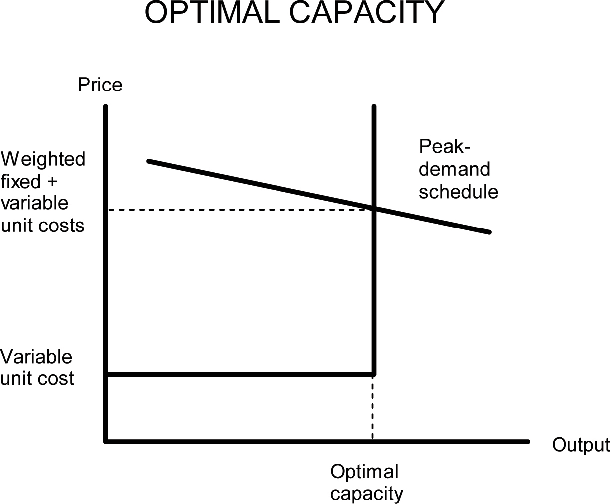
\includegraphics[width=1.\textwidth]{capacity/peak_load_opt}
    \caption{von der Fehr and Harbord (1994)}
    \label{fig:Daten 2004}            
\end{figure}
\end{column}

\begin{column} {0.6\textwidth}
\begin{itemize}
\item Optimal Capacity should be set such as to equate marginal benefits and costs from one unit of capacity
\end{itemize}

\begin{equation}
	c=(p^p-v)*\pi
\end{equation}

{\small
\begin{tabbing}
whereby: \= $c$ \  \= per unit cost of capacity \\
\> $p^p$   \    \> peak period price  \\
\> $v$    \   \> variable costs \\
\> $\pi$    \    \> chance to pave a peak period
\end{tabbing}}

\begin{itemize}
\item Which is exactly what a perfectly competitive firm would do
\end {itemize}

\begin{itemize}
\item Note that we assume price rationing and no rationing costs
\end {itemize}

\end{column}
\end{columns}

\end{frame}
\begin{frame}

\frametitle{Distorted Incentives under imperfect Competition I}
\begin{columns}
\begin{column} {0.4\textwidth}

\begin{figure}[h]
\centering
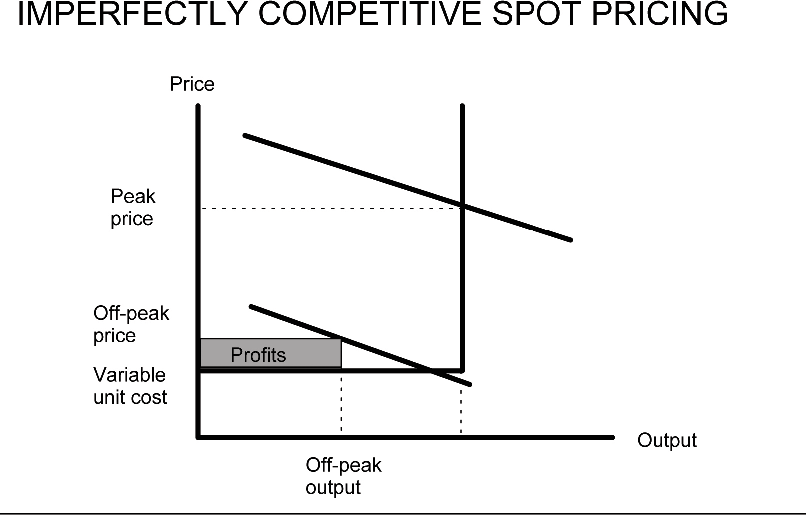
\includegraphics[width=1.\textwidth]{capacity/peak_load_toohigh}
    \caption{von der Fehr and Harbord (1994)}
    \label{fig:Daten 2004}            
\end{figure}
\end{column}

\begin{column} {0.6\textwidth}
\begin{itemize}
\item prices $>$ marginal costs in off peak periods 
\item additional incentive to invest by a possible gain during off peak periods if capacity allows to steal business
\end {itemize}
  
\begin{equation}
	1/2 (1-\pi) (p^{op}-v)
\end{equation} 
{\small
\begin{tabbing}
whereby: \= $p^{op}$ \  \= off peak price
\end{tabbing}}

\begin{itemize}
\item the social optimality condition is the same as before
\item distortion toward too much investment
\end {itemize}

\end{column}
\end{columns}
	

\end{frame}
\begin{frame}

\frametitle{Distorted Incentives under imperfect Competition II}
\begin{columns}
\begin{column} {0.4\textwidth}

\begin{figure}[h]
\centering
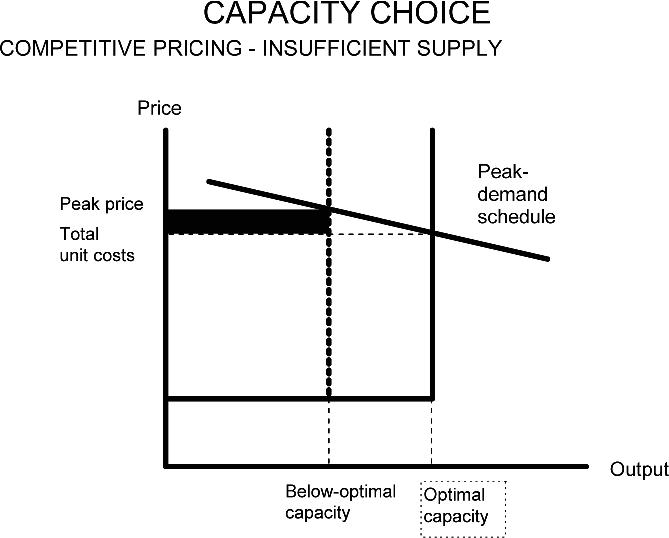
\includegraphics[width=1.\textwidth]{capacity/peak_load_insufficient}
    \caption{von der Fehr and Harbord (1994)}
   % \label{fig:Daten 2004}            
\end{figure}
\end{column}

\begin{column} {0.6\textwidth}
\begin{itemize}
\item there might be an incentive to cut investments to drive up the price in peak periods
\end {itemize}

\begin{equation}
\pi (w^p(K)+\frac{\partial w^p(K)}{\partial q}-v)
\end{equation}

{\small
\begin{tabbing}
\= $w^p$ \  \= peak period demand function \\
\> $K$   \    \> capacity
\end{tabbing}}

\begin{itemize}
\item as we switched to imperfect competition, the change in price induced by more capacity has to be accounted for
\item as this effect is negative, incentives to invest are distorted downwards
\end {itemize}

\end{column}
\end{columns}
	

\end{frame}

\subsection{Optimal Technology Mix}

\begin{frame}

\frametitle{The optimal Technology Mix I}
\begin{columns}
\begin{column} {0.4\textwidth}

\begin{figure}[h]
\centering
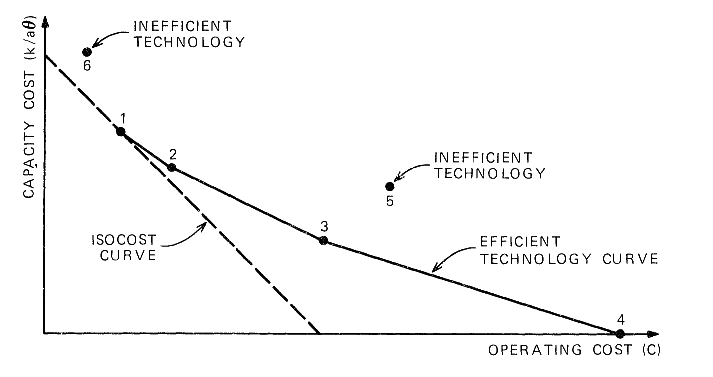
\includegraphics[width=1.\textwidth]{capacity/technology_choice_chow}
    \caption{Chau (1983)}
    \label{fig:Daten 2004}            
\end{figure}
\end{column}

\begin{column} {0.6\textwidth}
\begin{itemize}
\item how to choose the optimal technology?
\item different possible combinations of capacity and operating costs
\item by using a standard isocost line one could get the cheapest technology
\item does not work if demand is uncertain or variable
\item some idle capacity inevitable
\item less capital intensive technologies become attractive
\end {itemize}

\end{column}
\end{columns}

\end{frame}			
\begin{frame}

\frametitle{The optimal Technology Mix II}
\begin{columns}
\begin{column} {0.4\textwidth}

\begin{figure}[h]
\centering
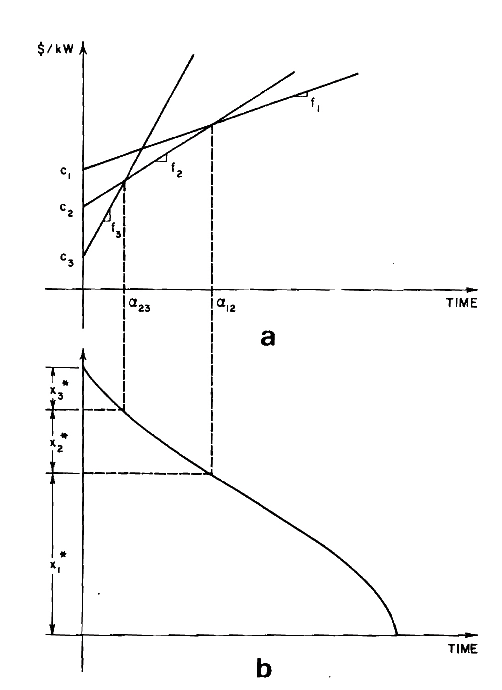
\includegraphics[width=1.\textwidth]{capacity/technology_choice_sherali}
    \caption{Chau (1983)}
    \label{fig:Daten 2004}            
\end{figure}
\end{column}

\begin{column} {0.6\textwidth}
\begin{itemize}
\item the load duration curve (\textbf{b}) plots the hours of the year ordered according to their energy demand
\item \textbf{(a)} shows three different cost curves each is cheaper for a certain yearly running time
\item technology 3 covers peak demand most efficiently 
\item but if it would run more than $\alpha_{23}$ hours of the year, technology two would be cheaper already
\item analogously, technology one is best used for base load
\end {itemize}

\end{column}
\end{columns}

\end{frame}	
%%% Local Variables: 
%%% mode: latex
%%% TeX-master: "../informs_puertorico"
%%% End: 
